\chapter{Vulnerabilities}
In this chapter we'll take a deeper look into vulnerabilities and the related attacks,
providing some examples and details.\nl

A dummy but instructive vulnerabilties classification distinguishes two major classes:
\begin{enumerate}
    \item \textbf{Local vulnerability} $\rightarrow$ vulnerability in a single \textit{module}.
    Even if the vulnerability needs other modules to be exploited, the defect it mostly depends on is in a single module, 
    and such kind of vulnerabilities can be removed by updating the modules they're dependant on.
    \item \textbf{Structural vulnerability} $\rightarrow$ a vulnerability which arises as a result of the composition of multiple modules.
    Also called \textit{emerging} vulnerability.
\end{enumerate}

\section{Local vulnerabilities}
A basic example of a local vulnerability, is \textbf{memory overflow},
particularly easy to exploit in software written in C, due to its memory management.
Basically, it is possible to \textit{inject code} in a small memory area by inserting more data than the actual available space.
It is common for many attacks to inject \textit{code} where the software expects \textit{data}.
Another known example is SQL injection.\nl

It is possible to inject code exploiting \textbf{stack overflow}.
stack memory areas start at the highest memory addresses and grow backwards, towards lower addresses.
\begin{center}
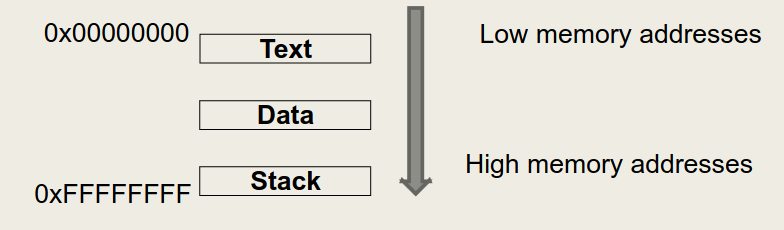
\includegraphics[width=0.5\textwidth]{images/stack_overflow.png}
\end{center}
Thus it is possible to inject fake stack frames and pointers to them in the \textit{data} area, using overflow and preventing segmentation faults.

\subsection{Address Space Layout Randomization ASLR}

(...)

\section{Structural Vulnerabilties}
Many attacks exploiting structural vulnerabilities were aimed to discover alive nodes in a network.
There is \textit{no control} on the fields of IP packets, thus senders are not authenticated.
A threat agent may send \textit{ECHO} messages using a broadcast address or to specific nodes to find out which are alive.

The \textit{Distributed \textbf{Denial of Service}} is performed by flooding a network with \textit{echo} messages,
making the bandwidth occupied by such messages and relative replies,
stopping the services running in such network.

A \textit{Slow Denial of Service}, instead, exploits collisions in a hash table to fill up memory and slow down performance of a Module.
\note{Is this a local vulnerability? Maybe not because it also depends by the possibility for the attacker to push input into the hash table.}

\section{Security Partial Views}
\subsection{Encryption}
According to Baiardi, \textbf{Encryption} \textit{simplifies} some \textbf{security} problems, but does \textbf{not} \textit{solve} them.
Encryption guarantees \textit{Confidentiality}, and sometimes \textit{Integrity}, but \textbf{not} \textit{Availability}.
Some claim that encryption solves security, but it must be taken into account that the operating system of a module may not provide a way to protect the encryption keys properly.

\subsection{Authentication}
Most security problem require three problems to be solved:
\begin{enumerate}
    \item User identification
    \item Resource identification
    \item Analysis of access rights
\end{enumerate}
User identification is not sufficient, \textit{as some may say}, because it indicates which row of the \textbf{Access Control Matrix} to consider, but not how to actually use the matrix.

To provide authentication three classes are considered, and the well known two-factor authentication should pick factor from two of these:
\begin{enumerate}
    \item \textit{Something you \textbf{know}}: password, PIN, pet name
    \item \textit{Something you \textbf{own}}: smartphone, credit card, token
    \item \textit{Something you \textbf{have}}: biometric features, i.e. fingerprint, voice, retina
\end{enumerate}

